% Slide 14: RNN 
\begin{frame}{}
  \LARGE RNN : \textbf{Architecture}
\end{frame}

% Visual from source PDF (page 14)
\begin{frame}{RNN Architecture: Unrolled View}
  \begin{columns}[c]
    \begin{column}{0.52\textwidth}
      \textbf{Unrolled RNN:} \\
      An RNN is essentially a chain of repeating neural network modules, one for each time step.
      \vspace{0.5em}
      
      \textbf{Each time step shares the same parameters:}
      \begin{itemize}
        \item[\textcolor{red}{$\blacktriangleright$}] Input $x_t$
        \item[\textcolor{red}{$\blacktriangleright$}] Hidden state $h_t$
        \item[\textcolor{red}{$\blacktriangleright$}] Output $y_t$
      \end{itemize}
      
      \textcolor{blue}{\textbf{Key Idea}} \\
      Temporal representation without increasing parameter count!
    \end{column}
    \begin{column}{0.48\textwidth}
      \centering
      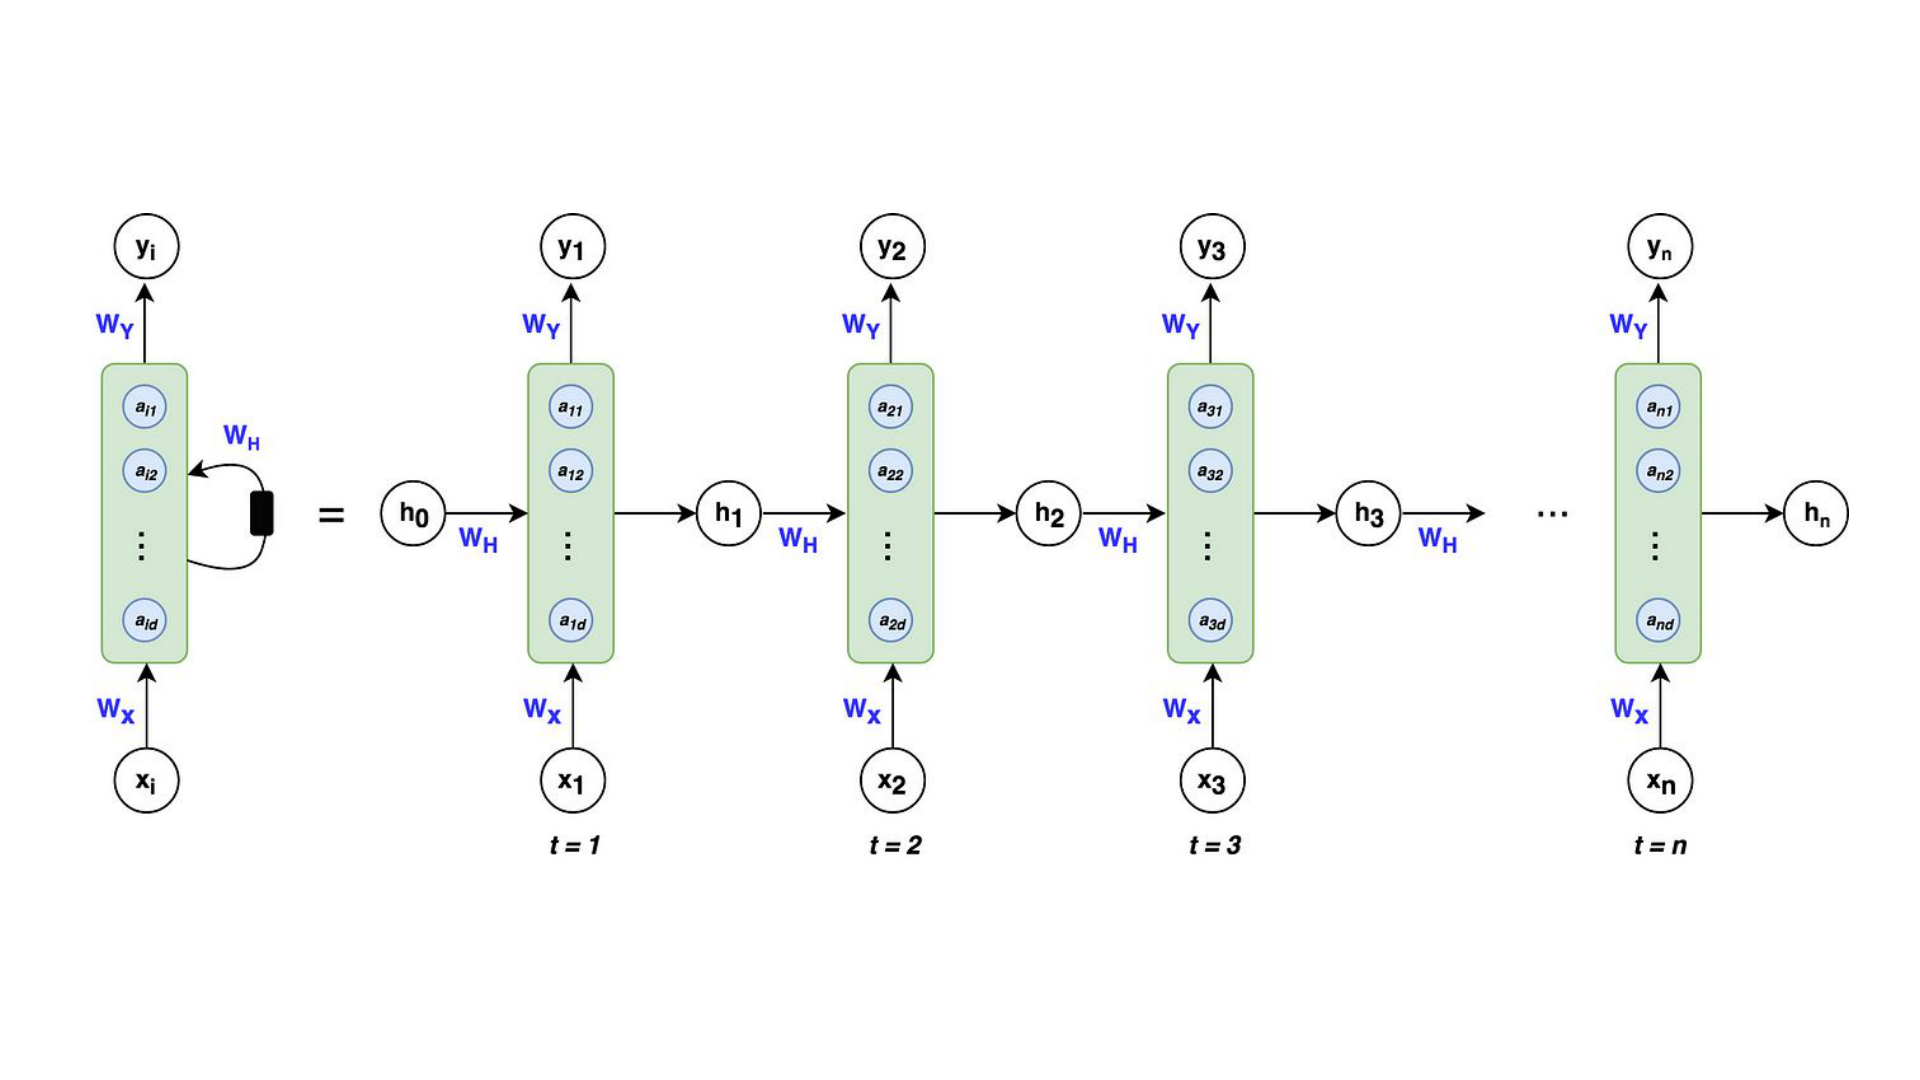
\includegraphics[width=0.99\linewidth,keepaspectratio]{assets/Lecture-3_Recurrent_Neural_Networks/pdf_page_002.png}
    \end{column}
  \end{columns}
\end{frame}

% ---------------------------------------------------------------------------
% Remaining slides from \texttt{Lecture-3\_Recurrent\_Neural\_Networks.pptx.pdf}
% (full-page raster). Omitted page numbers already appear above as text slides
% or as \texttt{slide\_002.png} / \texttt{slide\_006.png} / \texttt{slide\_014.png}.
% ---------------------------------------------------------------------------

\begin{frame}{Vanilla Neural Network}
  \centering
  
\includegraphics[width=0.9\paperwidth,height=0.8\paperheight,keepaspectratio]{assets/Lecture-3_Recurrent_Neural_Networks/pdf_page_016.png}
\end{frame}

\begin{frame}{One to One}
  \centering
  
\includegraphics[width=0.8\paperwidth,height=0.8\paperheight,keepaspectratio]{assets/Lecture-3_Recurrent_Neural_Networks/pdf_page_017.png}
\end{frame}

\begin{frame}{RNN: Process Sequences}
  \centering
  
\includegraphics[width=0.8\paperwidth,height=0.8\paperheight,keepaspectratio]{assets/Lecture-3_Recurrent_Neural_Networks/pdf_page_018.png}
\end{frame}

\begin{frame}{One to Many}
  \centering
  
\includegraphics[width=0.9\paperwidth,height=0.95\paperheight,keepaspectratio]{assets/Lecture-3_Recurrent_Neural_Networks/pdf_page_019.png}
\end{frame}

\begin{frame}{RNN: Process Sequences}
  \centering
  
\includegraphics[width=0.9\paperwidth,height=0.95\paperheight,keepaspectratio]{assets/Lecture-3_Recurrent_Neural_Networks/pdf_page_020.png}
\end{frame}

\begin{frame}{Many to One}
  \centering
  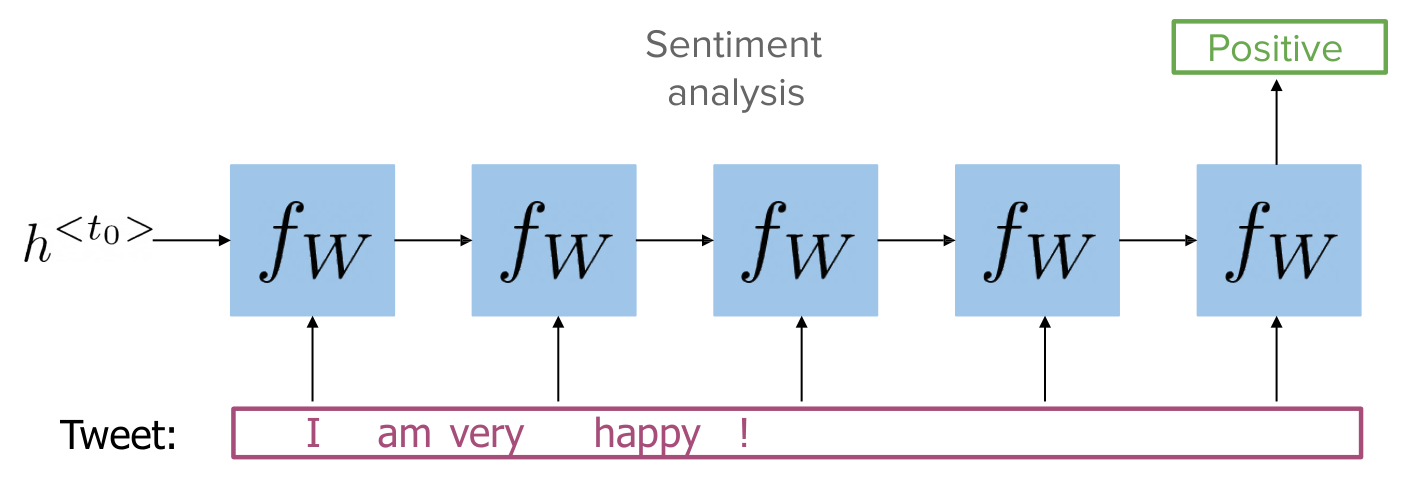
\includegraphics[width=0.9\paperwidth,height=0.95\paperheight,keepaspectratio]{assets/Lecture-3_Recurrent_Neural_Networks/pdf_page_021.png}
\end{frame}

\begin{frame}{RNN: Process Sequences}
  \centering
  
\includegraphics[width=0.9\paperwidth,height=0.95\paperheight,keepaspectratio]{assets/Lecture-3_Recurrent_Neural_Networks/pdf_page_022.png}
\end{frame}

\begin{frame}{Many to Many}
  \centering
  
\includegraphics[width=0.9\paperwidth,height=0.95\paperheight,keepaspectratio]{assets/Lecture-3_Recurrent_Neural_Networks/pdf_page_023.png}
\end{frame}

\begin{frame}{RNN: Process Sequences}
  \centering
  
\includegraphics[width=0.9\paperwidth,height=0.95\paperheight,keepaspectratio]{assets/Lecture-3_Recurrent_Neural_Networks/pdf_page_024.png}
\end{frame}

\begin{frame}{Recurrent Neural Network}
  \centering
  
\includegraphics[width=0.9\paperwidth,height=0.85\paperheight,keepaspectratio]{assets/Lecture-3_Recurrent_Neural_Networks/pdf_page_025.png}
\end{frame}

\begin{frame}{Unrolled RNN}
  \centering
  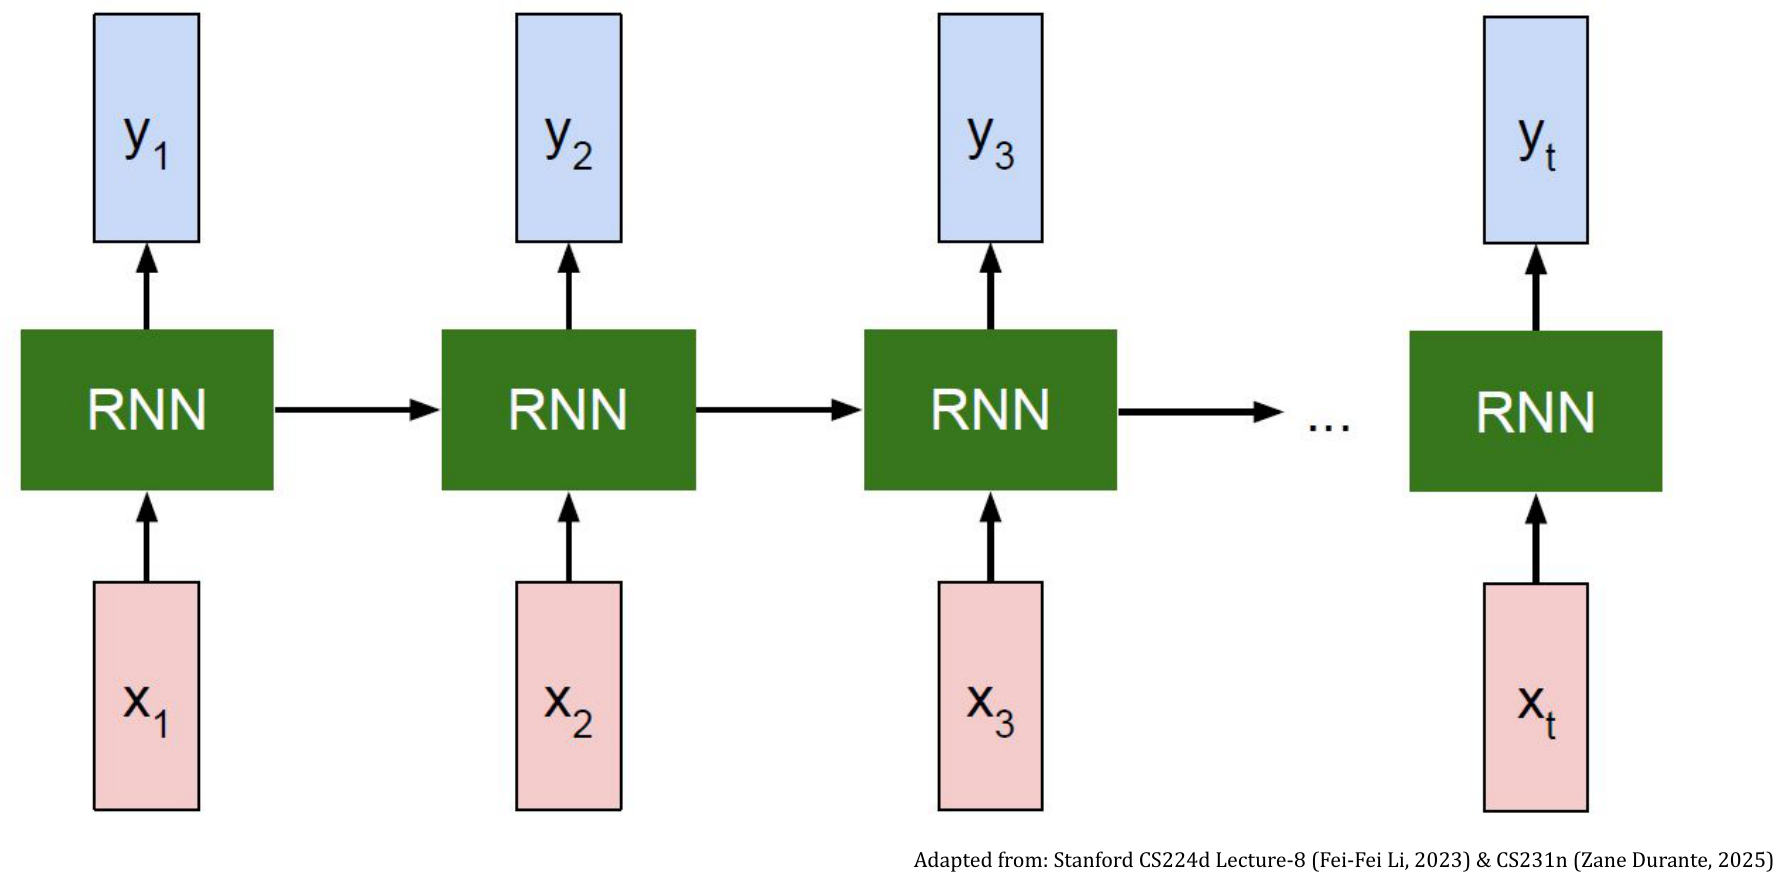
\includegraphics[width=0.9\paperwidth,height=0.95\paperheight,keepaspectratio]{assets/Lecture-3_Recurrent_Neural_Networks/pdf_page_026.png}
\end{frame}

\begin{frame}{}
  \LARGE RNN : \textbf{Mathematical Formulations}
\end{frame}

\begin{frame}{Math in Simple RNNs}
  \begin{itemize}
  \item How RNNs propagate information (Through time!)
  \item How RNNs make predictions
  \end{itemize}
\end{frame}

\begin{frame}{A Vanilla RNN}
  \centering
  
\includegraphics[width=0.9\paperwidth,height=0.82\paperheight,keepaspectratio]{assets/Lecture-3_Recurrent_Neural_Networks/pdf_page_029.png}

  \vspace{0.3em}
  {\footnotesize Here $g(\cdot)$ denotes the activation function (e.g.\ $\tanh$ or $\sigma$) --- a generic symbol for whichever nonlinearity is applied.}
\end{frame}

\begin{frame}{A Vanilla RNN}
  \centering
  
\includegraphics[width=0.9\paperwidth,height=0.82\paperheight,keepaspectratio]{assets/Lecture-3_Recurrent_Neural_Networks/pdf_page_030.png}

  \vspace{0.3em}
  {\footnotesize $g(\cdot)$ is the activation function (e.g.\ $\tanh$ or $\sigma$).}
\end{frame}

\begin{frame}{A Vanilla RNN}
  \begin{columns}[c]
    \column{0.4\textwidth}
      \centering
      % RNN Diagram from original image
      
\includegraphics[width=\textwidth,height=0.8\textheight,keepaspectratio]{assets/Lecture-3_Recurrent_Neural_Networks/pdf_page_031.png}
    \column{0.6\textwidth}
      \small
      \textbf{The state consists of a single ``hidden'' vector $\mathbf{h}$:}
      \vspace{0.5em}
      \begin{align*}
        \mathbf{h}_t &= f_W(\mathbf{h}_{t-1}, \mathbf{x}_t)
        \\
        \mathbf{h}_t &= \tanh(W_{hh}\mathbf{h}_{t-1} + W_{xh}\mathbf{x}_t)
        \\
        \mathbf{y}_t &= W_{hy} \mathbf{h}_t
      \end{align*}
      \vspace{0.5em}
      \begin{itemize}
        \item Sometimes called a ``Vanilla RNN'' or an \emph{Elman RNN} after Prof. Jeffrey Elman.
      \end{itemize}
      {\scriptsize
      \textit{Adapted from: Stanford CS224d Lectures (R. Socher), 2023 / CSD126 (Juan Durantez, 2023)}
      }
  \end{columns}
\end{frame}

\begin{frame}{}
  \LARGE RNN : \textbf{Parameter Sharing}
\end{frame}

\begin{frame}{RNN: Computation Graph}
  \centering
  
\includegraphics[width=0.9\paperwidth,height=0.70\paperheight,keepaspectratio]{assets/Lecture-3_Recurrent_Neural_Networks/pdf_page_033.png}
\end{frame}

\begin{frame}{RNN: Computation Graph}
  \centering
  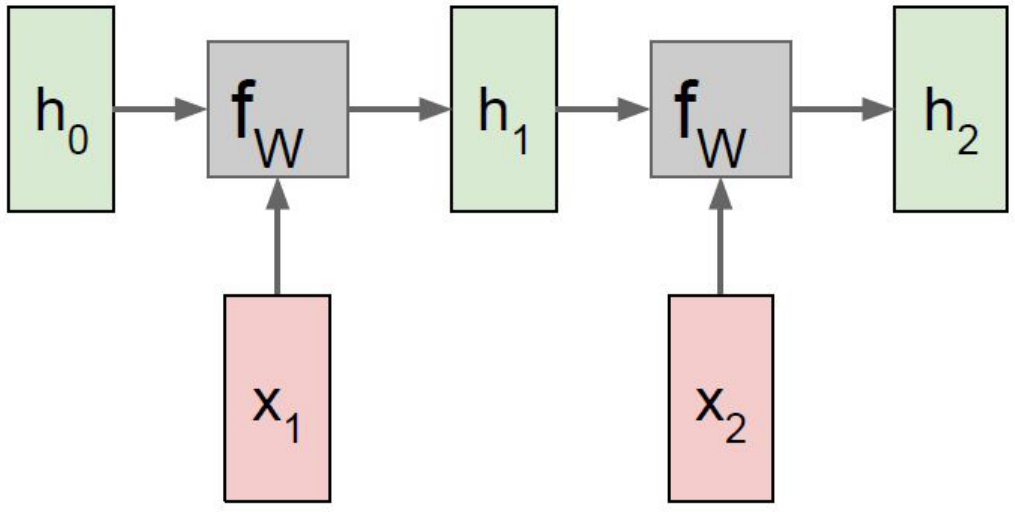
\includegraphics[width=0.9\paperwidth,height=0.85\paperheight,keepaspectratio]{assets/Lecture-3_Recurrent_Neural_Networks/pdf_page_034.png}
\end{frame}

\begin{frame}{RNN: Computation Graph}
  \centering
  
\includegraphics[width=0.9\paperwidth,height=0.95\paperheight,keepaspectratio]{assets/Lecture-3_Recurrent_Neural_Networks/pdf_page_035.png}
\end{frame}

\begin{frame}{RNN: Computation Graph}
  \centering
  
\includegraphics[width=0.9\paperwidth,height=0.95\paperheight,keepaspectratio]{assets/Lecture-3_Recurrent_Neural_Networks/pdf_page_036.png}
\end{frame}

\begin{frame}{RNN Computation Graph - Many to Many}
  \centering
  
\includegraphics[width=0.9\paperwidth,height=0.95\paperheight,keepaspectratio]{assets/Lecture-3_Recurrent_Neural_Networks/pdf_page_037.png}
\end{frame}

\begin{frame}{RNN Computation Graph - Many to Many}
  \centering
  
\includegraphics[width=0.9\paperwidth,height=0.95\paperheight,keepaspectratio]{assets/Lecture-3_Recurrent_Neural_Networks/pdf_page_038.png}
\end{frame}

\begin{frame}{RNN Computation Graph - Many to Many}
  \centering
  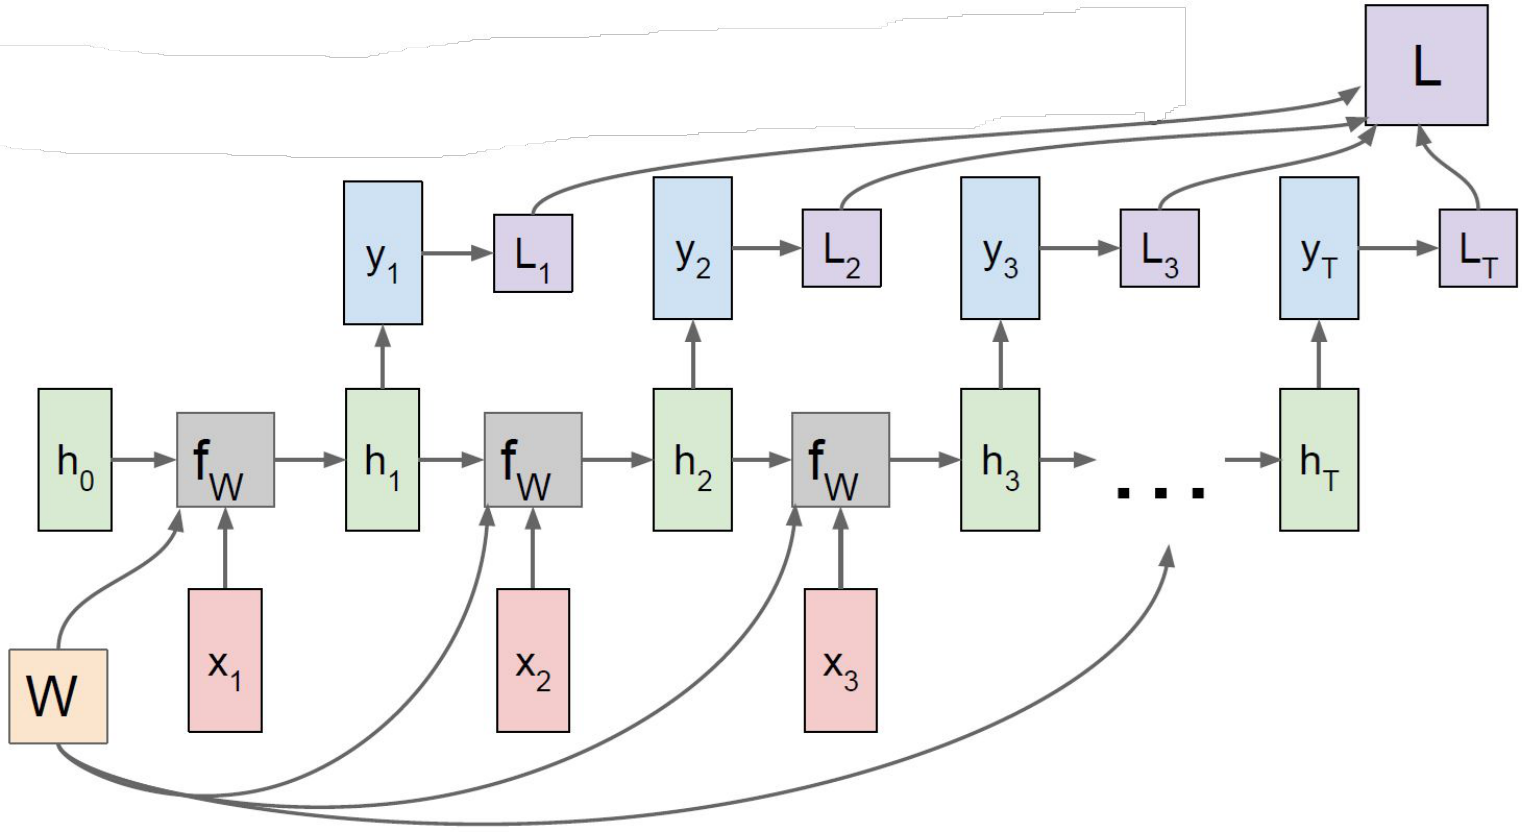
\includegraphics[width=0.9\paperwidth,height=0.95\paperheight,keepaspectratio]{assets/Lecture-3_Recurrent_Neural_Networks/pdf_page_039.png}
\end{frame}
